\documentclass[12pt,reqno,final,pdftex]{amsart}\usepackage[]{graphicx}\usepackage[]{color}
%% maxwidth is the original width if it is less than linewidth
%% otherwise use linewidth (to make sure the graphics do not exceed the margin)
\makeatletter
\def\maxwidth{ %
  \ifdim\Gin@nat@width>\linewidth
    \linewidth
  \else
    \Gin@nat@width
  \fi
}
\makeatother

\definecolor{fgcolor}{rgb}{0.345, 0.345, 0.345}
\newcommand{\hlnum}[1]{\textcolor[rgb]{0.686,0.059,0.569}{#1}}%
\newcommand{\hlstr}[1]{\textcolor[rgb]{0.192,0.494,0.8}{#1}}%
\newcommand{\hlcom}[1]{\textcolor[rgb]{0.678,0.584,0.686}{\textit{#1}}}%
\newcommand{\hlopt}[1]{\textcolor[rgb]{0,0,0}{#1}}%
\newcommand{\hlstd}[1]{\textcolor[rgb]{0.345,0.345,0.345}{#1}}%
\newcommand{\hlkwa}[1]{\textcolor[rgb]{0.161,0.373,0.58}{\textbf{#1}}}%
\newcommand{\hlkwb}[1]{\textcolor[rgb]{0.69,0.353,0.396}{#1}}%
\newcommand{\hlkwc}[1]{\textcolor[rgb]{0.333,0.667,0.333}{#1}}%
\newcommand{\hlkwd}[1]{\textcolor[rgb]{0.737,0.353,0.396}{\textbf{#1}}}%

\usepackage{framed}
\makeatletter
\newenvironment{kframe}{%
 \def\at@end@of@kframe{}%
 \ifinner\ifhmode%
  \def\at@end@of@kframe{\end{minipage}}%
  \begin{minipage}{\columnwidth}%
 \fi\fi%
 \def\FrameCommand##1{\hskip\@totalleftmargin \hskip-\fboxsep
 \colorbox{shadecolor}{##1}\hskip-\fboxsep
     % There is no \\@totalrightmargin, so:
     \hskip-\linewidth \hskip-\@totalleftmargin \hskip\columnwidth}%
 \MakeFramed {\advance\hsize-\width
   \@totalleftmargin\z@ \linewidth\hsize
   \@setminipage}}%
 {\par\unskip\endMakeFramed%
 \at@end@of@kframe}
\makeatother

\definecolor{shadecolor}{rgb}{.97, .97, .97}
\definecolor{messagecolor}{rgb}{0, 0, 0}
\definecolor{warningcolor}{rgb}{1, 0, 1}
\definecolor{errorcolor}{rgb}{1, 0, 0}
\newenvironment{knitrout}{}{} % an empty environment to be redefined in TeX

\usepackage{alltt}
%% DO NOT DELETE OR CHANGE THE FOLLOWING TWO LINES!
%% $Revision$
%% $Date$
\usepackage[round,sort,elide]{natbib}
\usepackage{graphicx}
\usepackage{times}
\usepackage{rotating}
\usepackage{subfig}
\usepackage{color}
\newcommand{\aak}[1]{\textcolor{cyan}{#1}}
\newcommand{\mab}[1]{\textcolor{red}{#1}}
\newcommand{\cec}[1]{\textcolor{blue}{#1}}

\setlength{\textwidth}{6.25in}
\setlength{\textheight}{8.75in}
\setlength{\evensidemargin}{0in}
\setlength{\oddsidemargin}{0in}
\setlength{\topmargin}{-.35in}
\setlength{\parskip}{.1in}
\setlength{\parindent}{0.3in}

%% cleveref must be last loaded package
\usepackage[sort&compress]{cleveref}
\newcommand{\crefrangeconjunction}{--}
\crefname{figure}{Fig.}{Figs.}
\Crefname{figure}{Fig.}{Figs.}
\crefname{table}{Table}{Tables}
\Crefname{table}{Tab.}{Tables}
\crefname{equation}{Eq.}{Eqs.}
\Crefname{equation}{Eq.}{Eqs.}
\crefname{appendix}{Appendix}{Appendices}
\Crefname{appendix}{Appendix}{Appendices}
\creflabelformat{equation}{#2#1#3}

\theoremstyle{plain}
\newtheorem{thm}{Theorem}
\newtheorem{corol}[thm]{Corollary}
\newtheorem{prop}[thm]{Proposition}
\newtheorem{lemma}[thm]{Lemma}
\newtheorem{defn}[thm]{Definition}
\newtheorem{hyp}[thm]{Hypothesis}
\newtheorem{example}[thm]{Example}
\newtheorem{conj}[thm]{Conjecture}
\newtheorem{algorithm}[thm]{Algorithm}
\newtheorem{remark}{Remark}
\renewcommand\thethm{\arabic{thm}}
\renewcommand{\theremark}{}

\numberwithin{equation}{part}
\renewcommand\theequation{\arabic{equation}}
\renewcommand\thesection{\arabic{section}}
\renewcommand\thesubsection{\thesection.\arabic{subsection}}
\renewcommand\thefigure{\arabic{figure}}
\renewcommand\thetable{\arabic{table}}
\renewcommand\thefootnote{\arabic{footnote}}

\newcommand\scinot[2]{$#1 \times 10^{#2}$}
\newcommand{\code}[1]{\texttt{#1}}
\newcommand{\pkg}[1]{\textsf{#1}}
\newcommand{\dlta}[1]{{\Delta}{#1}}
\newcommand{\Prob}[1]{\mathbb{P}\left[#1\right]}
\newcommand{\Expect}[1]{\mathbb{E}\left[#1\right]}
\newcommand{\Var}[1]{\mathrm{Var}\left[#1\right]}
\newcommand{\dd}[1]{\mathrm{d}{#1}}
\newcommand{\citetpos}[1]{\citeauthor{#1}'s \citeyearpar{#1}}
\IfFileExists{upquote.sty}{\usepackage{upquote}}{}
\begin{document}



\section*{Fitting the growth and reproduction trajectories of uninfected animals}
For this fitting, I need to use parameter values that make more sense for \emph{Daphnia dentifera}.
Hall et al. 2009 report that the mass of the host is $W=\alpha L^3$, where $\alpha=1.8\times 10^{-3}$ mgC mm$^{-3}$, and they assume (Appendix A) that half of the measured dry mass is carbon.
$L$ is the observed length, rather than the ``structural'' length of DEB theory; Spencer's formulation of the standard DEB model didn't involve the structural length, so this parameter wasn't needed.
In other words, $\alpha$ was estimated using observed dry weights $W$, observed lengths $L$, and an assumption that $W/2$ is the carbon mass of the host.

This is slightly different than what I have been doing, but is not incompatible with it.
I had assumed that observed mass $W_{obs} = W + E$, where $W$ is the ``structural'' mass and $E$ is the reserves, and that observed length was $L_{obs} = \xi W_{obs}^q$, where $\xi$ and $q$ are based on a regression of observed weight on observed length.
I then assumed that ``structural length'' $L$ was equal to $W^{1/3}$.
Basically, all I need to do is assume that $\xi=\alpha$ and $q=3$ and I will have recovered more or less the same parameterization.

I need better values from Spencer et al. for some of the parameters, so for my first attempt at fitting Cat's data for uninfected animals, I fixed $E_R = 1.51 \times 10^{-3}$, the initial biomass as $W+E = 0.00225$, and the biomass at maturity as 0.005.
I also fixed $v=10$ for the fitting.

The results are not particularly encouraging, frankly (Fig. \ref{fig:Cat-fits-1}).
The parameters are fairly tightly estimated at the highest likelihood parameter sets; in particular, $\rho=0.15$, $\kappa=0.077$, and $L_{obs}$ = 0.088.
However, that $\kappa$ value is much too low to make biological sense.
Neither $f_h$ nor $k_m$ are well-identified in the very highest likelihood parameter sets: for parameters sets within 1 log-likelihood unit of the maximum, $f_h$ varies between practically 0 and 10000 (although all but one estimate is less than 40, and two are essentially 0), while $k_m$ varies between essentially 0 and 0.008 (which is likely much too small).
There is also a very strong positive correlation between the estimates of $\kappa$ and $k_m$ that I haven't noticed before in the simulation-recovery fits.

The fact that the data seem to want $f_h=0$, implying food-independent feeding, is interesting/strange.
I cannot really explain why that should be favored.
\begin{knitrout}\scriptsize
\definecolor{shadecolor}{rgb}{0.969, 0.969, 0.969}\color{fgcolor}\begin{figure}

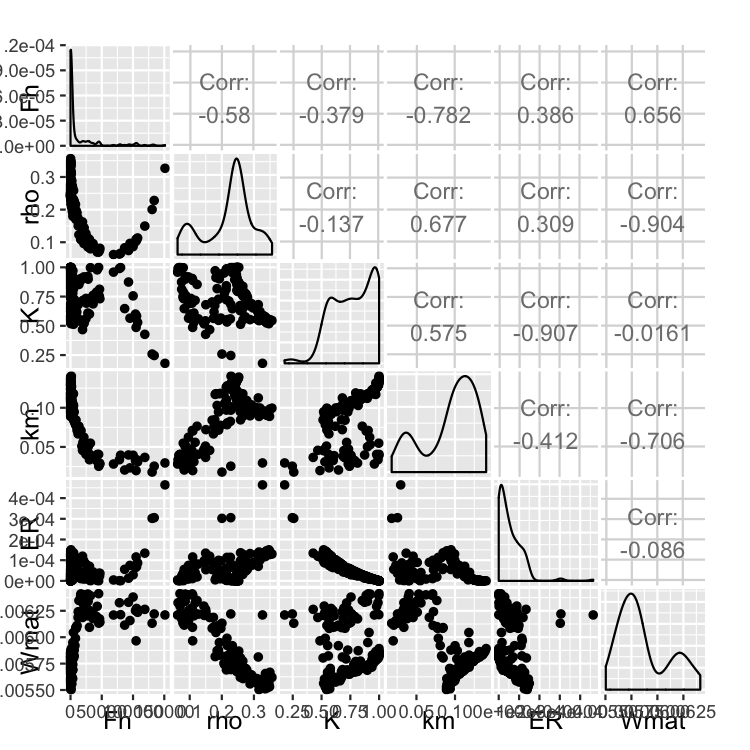
\includegraphics[width=\linewidth]{figure/Cat-fits-1-1} \hfill{}

\caption[Pairwise plot of parameter estimates from fitting Cat's growth and reproduction dataset]{Pairwise plot of parameter estimates from fitting Cat's growth and reproduction dataset.}\label{fig:Cat-fits-1}
\end{figure}


\end{knitrout}

I think the best thing to do is to try fixing $f_h$ at different values, and see how that affects the other parameter estimates.
Although I doubt if there is a parameter set with a higher likelihood that was overlooked by the algorithm, my sense is that it may be that the likelihood surface is quite flat, so $f_h$ can run off towards 0, dragging all of the other parameter estimates with it.
The profile likelihood will be very informative in this regard.

Suprisingly, the profile likelihood suggests that, indeed, the likelihood does increase in the direction of smaller $f_h$ values (Fig. \ref{fig:Cat-profile-lik-fh}).
You can see some interesting patterns in Fig. \ref{fig:Cat-profile-lik-fh}.
This figure shows all of the parameter estimates within two log-likelihood units of the maximum for each value of $f_h$.
You can see that there are ``lines'' showing particular relationships between, e.g., $\rho$ and $f_h$ and the log-likelihood and $f_h$ suggesting multiple fitness peaks with different scaling relationships between the variables.
\begin{knitrout}\scriptsize
\definecolor{shadecolor}{rgb}{0.969, 0.969, 0.969}\color{fgcolor}\begin{figure}

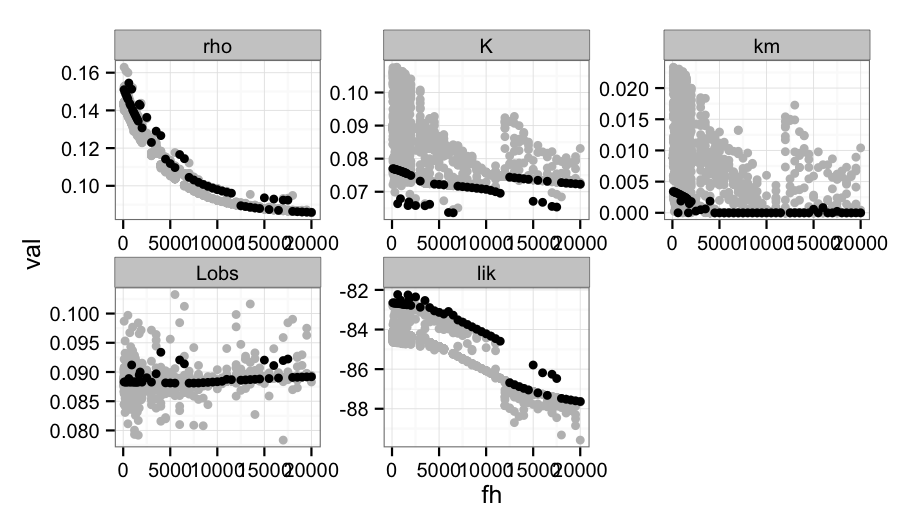
\includegraphics[width=\linewidth]{figure/Cat-profile-lik-fh-1} \hfill{}

\caption[Profile likelihood for ]{Profile likelihood for $f_h$ showing the best-fitting parameter estimates for Cat's uninfected \emph{Daphnia} as $f_h$ is varied.}\label{fig:Cat-profile-lik-fh}
\end{figure}


\end{knitrout}

These multiple likelihood peaks can be seen in pairwise scatterplot of the parameter estimates, for example, for $f_h=9000$ (Fig. \ref{fig:fh9000}).
Note, in particular, in the density plot that there are multiple likelihood peaks and multiple density peaks for each parameter.

\begin{knitrout}\scriptsize
\definecolor{shadecolor}{rgb}{0.969, 0.969, 0.969}\color{fgcolor}\begin{figure}

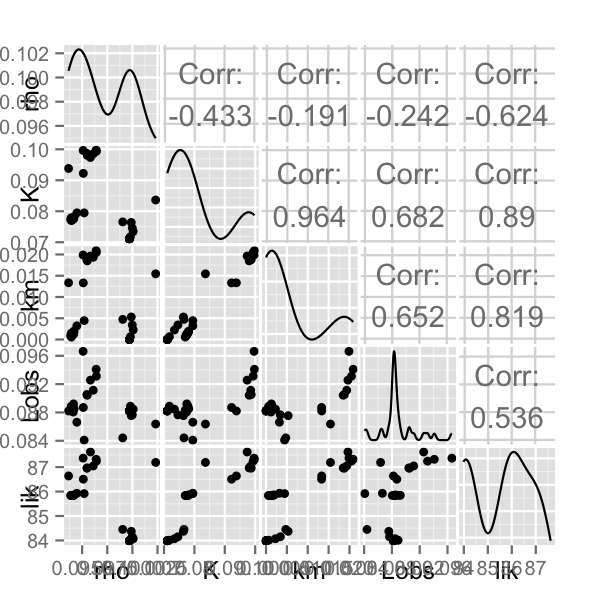
\includegraphics[width=0.5\textwidth]{figure/fh9000-1} \hfill{}

\caption[Scatterplot of parameter estimates for ]{Scatterplot of parameter estimates for $f_h=9000$.}\label{fig:fh9000}
\end{figure}


\end{knitrout}

The larger problem, however, is that these parameter values still seem highly biologically unrealistic and there is a very strong correlation between the estimates of $\kappa$ and $k_m$, suggesting that these might be difficult to independently estimate.
One concern that I have is that some of the fixed parameter estimates might be very far from the truth.
For example, the estimate of $\kappa$ being less than 0.1 indicates that the vast majority of energy is being shunted into reproduction.
This may be because the cost of reproduction $E_R$ is too high.
Recall that I was assuming $E_R=1.51 \times 10^{-3}$.
If this cost is equal to the mass of a neonate, this would suggest a neonate length of $(0.00151/0.0018)^{1/3}=0.94$mm, which is much too large.
I refit the model, assuming a cost of reproduction equal to $2.25 \times 10^{-4}$, which is equivalent to the mass of a 0.5mm neonate.
I also reduced the mass at maturity from 0.005 to 0.002, based on the estimate from Hall et al. 2009.
Finally, I fixed the value of $f_h$ at 2250 cells/ml, which is equivalent to 0.1mgC/L, the estimate reported in Hall et al. 2009.
Which those values fixed, I esimated only $\rho$, $\kappa$, $k_m$, and the observation error.
I constructed a profile likelihood over $v$, just to see if there was still no evidence for an effect of $v$ on the fits.
Fig. \ref{fig:v-profile-lik} shows the results.
It is clear that the parameter estimates are not much affected by $v$.
In fact, even taking $v$ as large as 10000 has no effect on the other parameter estimates, suggesting that the data really do support a reserve-less model.
The estimates of $\kappa$ and $k_m$, at any rate, seem more reasonable as well.
However, the estimate of $\rho$ is \emph{very} small, suggesting that the model is perhaps inadequate in some way.

\begin{knitrout}\scriptsize
\definecolor{shadecolor}{rgb}{0.969, 0.969, 0.969}\color{fgcolor}\begin{figure}

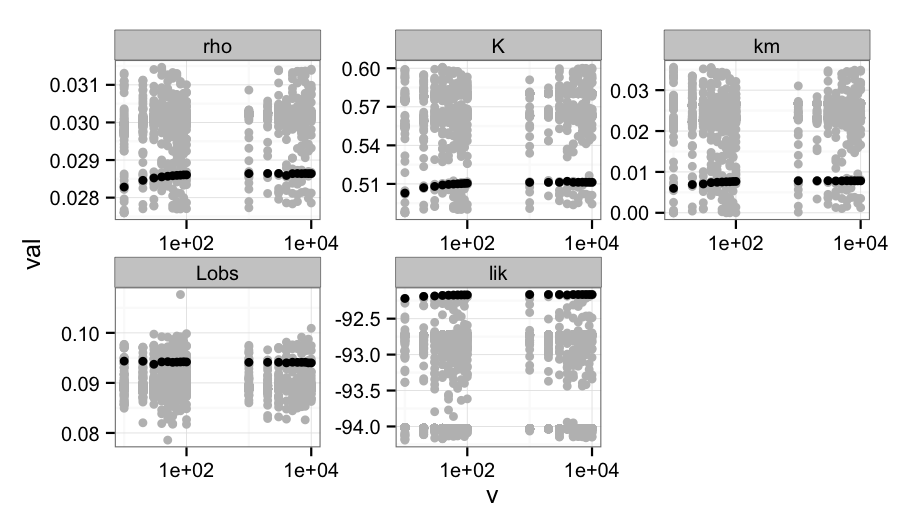
\includegraphics[width=\linewidth]{figure/v-profile-lik-1} \hfill{}

\caption[Parameter estimates as ]{Parameter estimates as $v$ is varied, when $f_h$ is fixed. The black point is the maximum likelihood parameter estimate.}\label{fig:v-profile-lik}
\end{figure}


\end{knitrout}

I want to point out that the seeming variation in the parameter estimates is a bit illusory.
Most of the parameter estimates are essentially lying directly under the maximum likelihood estimate, as can be seen in Fig. \ref{fig:estimates-v-10}, which shows the distribution of parameter estimates for $v=10$.
\begin{knitrout}\scriptsize
\definecolor{shadecolor}{rgb}{0.969, 0.969, 0.969}\color{fgcolor}\begin{figure}

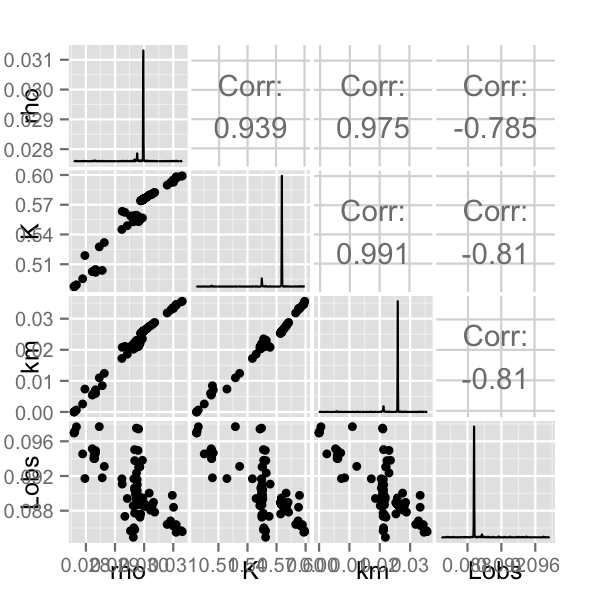
\includegraphics[width=0.75\textwidth]{figure/estimates-v-10-1} \hfill{}

\caption[Distribution of parameter estimates when ]{Distribution of parameter estimates when $v=10$ and $f_h$ is fixed.}\label{fig:estimates-v-10}
\end{figure}


\end{knitrout}
However, this distribution also reveals the \emph{very} strong correlations between the estimates of $\rho$, $\kappa$, and $k_m$.

\clearpage

I have a hypothesis both about why the estimate of $\rho$ is so low and why the estimates of $\rho$, $\kappa$, and $k_m$ are so strongly correlated.

As to the former question, recall the model that I am actually fitting to these data:
\begin{align}
\frac{dF}{dt} &= -I_{max} \frac{F}{f_h+F} L_{obs}^g \\
\frac{dE}{dt} &= \rho \epsilon V I_{max} \frac{F}{f_h+F} L_{obs}^g - p_C, \\
\frac{dW}{dt} &= \kappa~p_C - k_M~W, \\
\frac{dR}{dt} &= \frac{(1-\kappa)~p_C}{E_R}, \\
p_C &= E \left(\frac{\frac{v}{L} + k_m}{1+\frac{\kappa E}{W}}\right).
\end{align}
This model is missing a term for the cost of growth.
I am assuming that $x$ mgC of reserves allocated towards growth becomes $x$ mgC of new structural biomass.
In the standard DEB model, there is a conversion cost, such that growth in weight is actually:
\begin{equation}
\frac{dW}{dt} = \frac{\kappa~p_C - k_m~E_G~W}{E_G},
\end{equation}
and the mobilization rate is
\begin{equation}
p_C = E \left(\frac{\frac{v}{L} + k_m}{1+\frac{\kappa E}{E_G W}}\right).
\end{equation}
With this cost added in, the animals have to be more efficient at assimilation in order to meet all of the costs.

However, it turns out that adding this parameter doesn't make the estimation any easier or more reasonable, as you might expect based on the previous findings regarding the trade-offs between $\rho$ and $E_R$ (Fig. \ref{fig:with-EG-scatter}).
I fit the standard DEB model defined above to the data, assuming the same fixed parameter values but also attempting to estimate $E_G$.
Fig. \ref{fig:with-EG-scatter} shows the distribution of parameter estimates that were within 2 log-likelihood units of the maximum.
In addition to $\rho$ still being estimated as very small, most of the $\kappa$ estimates are near 1.
There are also clear and strong trade-offs between $\rho$ and $E_G$, as expected, as well as between $\rho$ and $\kappa$, $k_m$ and $E_G$, and $\kappa$ and $E_G$, and $\rho$ and $k_m$.
\begin{knitrout}\scriptsize
\definecolor{shadecolor}{rgb}{0.969, 0.969, 0.969}\color{fgcolor}\begin{figure}

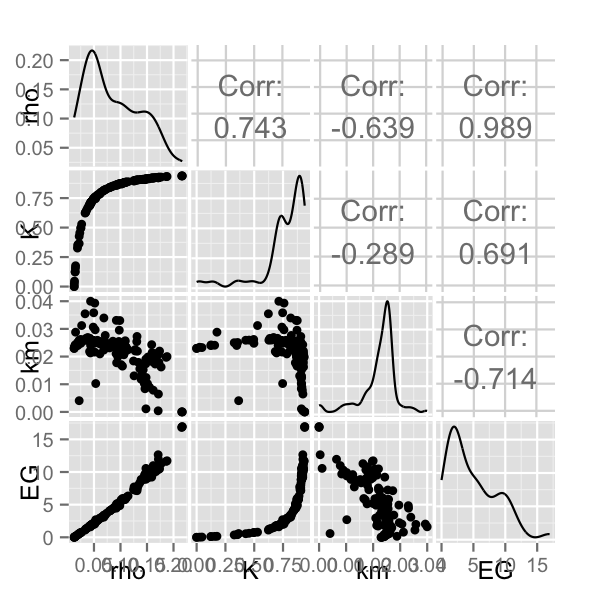
\includegraphics[width=0.75\textwidth]{figure/with-EG-scatter-1} \hfill{}

\caption[Correlations between the parameter estimates when ]{Correlations between the parameter estimates when $E_G$ is also estimated.}\label{fig:with-EG-scatter}
\end{figure}


\end{knitrout}

These results reinforce the question, raised earlier, about the correlation between parameter estimates.
This problem can be understood really simply.
If we take the results seriously that the value of $v$ has no effect on the dynamics, then we can assume that there is no reserve.
This leads to a model where assimilated resources are immediately allocated towards either growth and maintenance or reproduction.
This model makes the parameter estimation problem particularly evident.
In such a model, the dynamics of growth in structure $V$ and length $L$ are given as (note that I have simplified the expressions slightly):
\begin{align}
\frac{dV}{dt} &= \frac{\kappa}{E_G} \rho I_{max} \frac{F}{f_h+F} L^g - k_m V \text{ and} \\
\frac{dR}{dt} &= \frac{1-\kappa}{E_R} \rho I_{max} \frac{F}{f_h+F} L^g.
\end{align}
Clearly, I can play $\kappa$, $E_G$, and $E_R$ off against one another: for instance, the model can make $\kappa$ very small (so most resource going into reproduction), as long as $E_G$ is also small (so growth is cheap) and $E_R$ is large (so reproduction is expensive).
If I fix the estimate of $E_R$, as I have done before, the fitting algorithm is still free to play $\kappa$, $E_G$, and $\rho$ off against one another.

I think this is likely to be a \emph{very} general problem with these models, and almost certainly explains why the profile likelihood surfaces are so flat, as I have shown for $v$ and $f_h$: for any set value of a parameter ($E_G$, for example), the algorithm can play with the other parameters so as to achieve a similarly good fit to the data.
Fig. \ref{fig:profile-EG} shows a profile liklihood for $E_G$, where I have fixed $E_G$ and estimated $\rho$, $\kappa$, and $k_m$.
For any value of $E_G$, I am able to estimate the other parameters reasonably well.
Note, however, that I have already fixed $E_R$ (and $v$).
Fixing $E_G$ and $E_R$ limits the ability of the fitting algorithm to play the other parameters off against one another enough that most of the initial guesses converge on the same final estimate (recall, however, Fig. \ref{fig:estimates-v-10}, which implicitly fixed $E_G=1$ - although there were clear most-commonly supported estimates for $\rho$, $\kappa$, and $k_m$, nearby parameter sets definitely slide these around to achieve \emph{almost} as good a fit.
\begin{knitrout}\scriptsize
\definecolor{shadecolor}{rgb}{0.969, 0.969, 0.969}\color{fgcolor}\begin{figure}

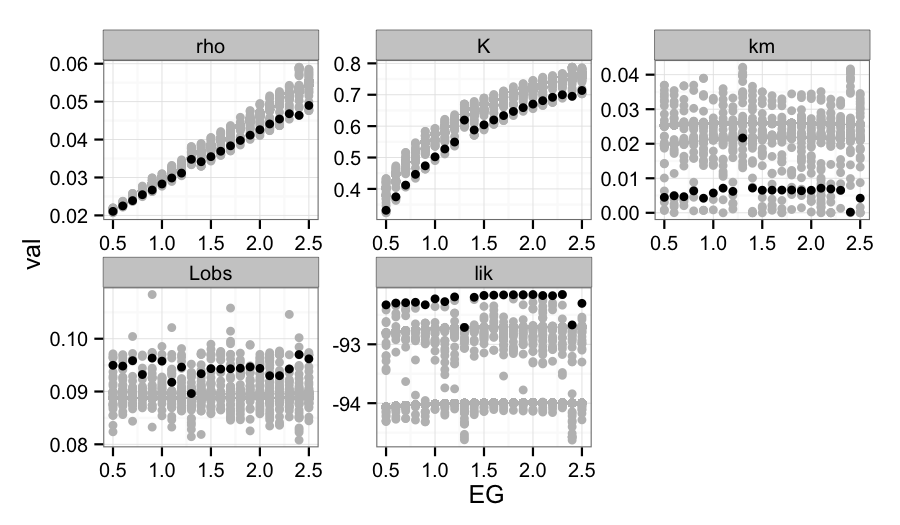
\includegraphics[width=\linewidth]{figure/profile-EG-1} \hfill{}

\caption[Profile likelihood over ]{Profile likelihood over $E_G$.}\label{fig:profile-EG}
\end{figure}


\end{knitrout}

The question is to what extent this problem can be addressed.
One possibility is to nondimensionalize the model, hopefully revealing important (and independent) parameter combinations that are critical to the model dynamics.

To that end, let's take a look at the standard DEB model again.
Here, I have replaced $W$ with $V$ to be totally consistent with the standard DEB model.
The volume of the container is given by $\mathcal{V}$.
\begin{align}
\frac{dF}{dt} &= -I_{max} \frac{F}{f_h+F} L_{obs}^g \\
\frac{dE}{dt} &= \rho \epsilon \mathcal{V} I_{max} \frac{F}{f_h+F} L_{obs}^g - p_C, \\
\frac{dV}{dt} &= \frac{\kappa~p_C - k_m~E_G~V}{E_G}, \\
\frac{dR}{dt} &= \frac{(1-\kappa)~p_C}{E_R}, \\
p_C &= E \left(\frac{\frac{v}{L} + k_m}{1+\frac{\kappa E}{E_G V}}\right).
\end{align}

The presence of the $E/V$ term in the denominator is suggestive: rather than working with a model parameterized in terms of $E$ and $V$, I am going to work instead on a model parameterized in terms of $E/V$ and $L$.
It turns out that this will be much more convenient for me in the long run, and standard DEB theory often works with the variable $E/V$, which is defined as the ``reserve density.''
I will define the new variable $W = E/V$.
Applying the chain rule, the dynamics of $W=E/V$ are
\begin{equation}
\frac{dW}{dt} = \frac{d(E/V)}{dt} = \frac{1}{V(t)}\frac{dE}{dt} - \frac{E(t)}{V(t)^2}\frac{dV}{dt}
\end{equation}
If you plug in the expressions for $dE/dt$ and $dV/dt$, you end up with the dynamics of the variable $W$ as
\begin{equation}
\frac{dW}{dt} = \rho \epsilon \mathcal{V} I_{max} \frac{F}{f_h+F} \frac{L^g}{V} - W \frac{v}{L},
\end{equation}
which is a very simple expression that actually eliminates a lot of the parameters already.
Note that I have also made the simplifying assumption that ``structural length'' $L$ and the observed length $L_{obs}$ are actually the same.

To find the equation for the dynamics of length, we need a way to convert length (which is in mm) to structural volume $V$.
A length-dry weight regression should be almost exactly converting length to structural volume, since the drying process would probably remove most of the weight that was tied up in reserve.
As such, we have that $V = \xi L^q$, and
\begin{equation}
\frac{dL}{dt} = \frac{1}{q \xi L^{q-1}}\frac{dV}{dt}.
\end{equation}
Simplifying, I have that
\begin{equation}\label{eq:length}
\frac{dL}{dt} = \frac{L}{q}\left(\frac{\frac{\kappa}{E_G}W\frac{v}{L} - k_m}{1 + \frac{\kappa}{E_G}W}\right).
\end{equation}

We can use this length-weight regression to eliminate $V$ from the equation for $dW/dt$ as well:
\begin{equation}\label{eq:reserve-density}
\frac{dW}{dt} = \rho \epsilon \mathcal{V} I_{max} \frac{F}{f_h+F} \frac{L^g}{\xi L^{q}} - W \frac{v}{L}.
\end{equation}

Note that equations \ref{eq:length} and \ref{eq:reserve-density} make sense together.
The reserve density $W$ increases through ingestion and is depleted through the mobilization of reserve to fuel growth and reproduction by an amount $W \frac{v}{L}$.
This shows up in the numerator of $dL/dt$, weighted by the fractional allocation to growth $\kappa$ and the cost of growth $E_G$.
There is subtraction due to maintenance $k_m$ and than a normalization $1 + \kappa W/E_G$ that comes from the reserve mobilization equation.

A simple examination of these two equations reveals right away that neither $\kappa$ nor $E_G$ by itself influences the dynamics of the system, only their combination $\kappa/E_G$.
Since $\kappa$ is a fraction between 0 and 1 and $E_G$ is the conversion cost converting mgC of reserve into mgC of structure, this is a dimensionless quantity.
The purpose of nondimensionalization is to find other dimensionless quantities that affect the system dynamics.

Essentially, I want to reparameterize the system, focusing on the dynamics of the dimensionless variables $f$, $w$, $\ell$, $r$, and $\tau$, rather than the dimensional variables $F$, $W$, $L$, $R$, and $t$.
Thus, define $F = \hat{f} f$, $W = \hat{w} w$, $L = \hat{\ell} \ell$, $R = \hat{r} r$, and $t = \hat{\tau} \tau$, where the ``hatted'' variables are combinations of parameters that scale the dimensionless stage variables, allowing you to exactly recover the dimensional dynamics.

Let's start with the food dynamics, and work from there.
The dimensional dynamics are
\begin{equation}
\frac{dF}{dt} = -I_{max}\frac{F}{f_h+F}L^g.
\end{equation}
The nondimensional dynamics are
\begin{equation}
\frac{df}{d\tau} = \frac{\hat{\tau}}{\hat{f}}\frac{dF}{dt}= \frac{\hat{\tau}}{\hat{f}}\left(-I_{max}\frac{\hat{f}f}{f_h + \hat{f}f}\hat{\ell}^g\ell^g\right).
\end{equation}
If I define $\hat{f} = f_h$, then I can simplify this equation to
\begin{equation}
\frac{df}{d\tau} = -\frac{\hat{\tau} I_{max} \hat{\ell}^g}{f_h} \frac{f}{1+f} \ell^g.
\end{equation}
Given that the units of $I_{max}$ are cells ml$^{-1}$ mm$^{-g}$ d$^{-1}$ and the units of $f_h$ are cells ml$^{-1}$, and that the units of $\hat{\ell}$ must be mm, if I define
\begin{equation*}
\hat{\tau} = \frac{f_h}{I_{max} \hat{\ell}^g},
\end{equation*}
then $\hat{\tau}$ will have the proper units.
This scaling means that we are measuring time in terms of ingestion, which makes sense given that ingestion sets all other processes.
Furthermore, since $f_h$, $I_{max}$ and $g$ are all known based on the feeding data, specifying the scaling of length automatically specifies the scaling of time.
This is important because, in order to fit the dimensionless model to data, I will have to estimate these scaling parameters.
With $\hat{\tau}$ specified, the dynamics of dimensionless food become
\begin{equation}
\frac{df}{d\tau} = -\frac{f}{1+f}\ell^g.
\end{equation}

Now let's consider the dynamics of dimensionless length:
\begin{equation*}
\frac{d\ell}{d\tau} = \frac{\hat{\tau}}{\hat{\ell}}\left(\frac{\hat{\ell}\ell}{q} \left(\frac{\frac{\kappa}{E_G}\hat{w}w\frac{v}{\hat{\ell}\ell}-k_m}{1+\frac{\kappa}{E_G}\hat{w}w} \right)\right)
\end{equation*}
If I define $\hat{w} = E_G/\kappa$ and $\hat{\ell} = v/k_m$ then this equation simplifies to
\begin{equation}
\frac{d\ell}{d\tau} = k_m \hat{\tau} \frac{\ell}{q}\left(\frac{\frac{w}{\ell}-1}{1+w}\right)
\end{equation}
Note that the combination $k_m \hat{\tau}$ will be dimensionless, since $k_m$ has units of 1/time and $\hat{\tau}$ has units of time.
I will define the dimensionless parameter $\alpha=k_m \hat{\tau}$.

The dynamics of dimensionless reserve density are
\begin{equation}
\frac{dw}{d\tau} = \frac{\hat{\tau}}{\hat{w}} \rho \epsilon \mathcal{V} I_{max} \frac{\hat{f}f}{f_h+\hat{f}f}\frac{\hat{\ell}^g\ell^g}{\xi\hat{\ell}^q\ell^q} - \frac{\hat{\tau}}{\hat{w}}\hat{w}w\frac{v}{\hat{\ell}\ell}
\end{equation}
Simplifying this equation, we have
\begin{equation}
\frac{dw}{d\tau} = \frac{\rho}{\hat{w}}\frac{f_h \epsilon \mathcal{V}}{\xi \hat{\ell}^q}\frac{f}{1+f}\ell^{g-q}-k_m\hat{\tau} \frac{w}{\ell}
\end{equation}
Note that the quantity $\phi=\frac{f_h \epsilon \mathcal{V}}{\xi \hat{\ell}^q}$ is dimensionless.
I could define a dimensionless quantity $\sigma = \frac{\rho}{\hat{w}}$ - however, that could be problematic when it comes time to do the fitting.
This is because I would be estimating both the value of $\sigma$ and the value of $\hat{w}$; both of these parameters could take on any positive value, but their product $\rho = \sigma \hat{w}$ is constrained to take only values between 0 and 1.
Because of that, it makes more sense to keep $\rho$ in the model as a dimensionless parameter to be estimated.
The dimensionless quantity $\alpha=k_m\hat{\tau}$ also appears in this equation.

Finally, we have the equation for egg production.
Note that $R$ is already dimensionless, as it is just a number.
I will also replace the $E$ in the mobilization equation $p_C$ with $E=W~V=W~\xi~L^q$, to focus on the variables we are actually interested in:
\begin{equation*}
\frac{dR}{d\tau} = \hat{\tau} \frac{1-\kappa}{E_R} \hat{w}w \xi \hat{\ell}^q\ell^q \left(\frac{\frac{v}{\hat{\ell}\ell} + k_m}{1 + \frac{\kappa}{E_G}\hat{w}w}\right)
\end{equation*}
This can also be simplified to
\begin{equation}
\frac{dR}{d\tau} = \frac{E_G}{E_R}\frac{1-\kappa}{\kappa}\xi\hat{\ell}^q k_m\hat{\tau} \ell^q \left(\frac{\frac{1}{\ell}+1}{1+w}\right).
\end{equation}
I will define the new parameter
\begin{equation}
\beta = \frac{E_G}{E_R}\frac{1-\kappa}{\kappa}\xi\hat{\ell}^q
\end{equation}
which is dimensionless (because $E_G$ is dimensionless, $E_R$ has units of mgC, $\kappa$ is dimensionless, $\xi$ has units of mgC mm$^{-q}$, and $\hat{\ell}^q$ has units of mm$^q$).

Putting all of these equations together, I have the dimensionless system:
\begin{align}
\frac{df}{d\tau} &= -\frac{f}{1+f}\ell^g, \\
\frac{dw}{d\tau} &= \frac{\rho\phi}{\hat{w}}\frac{f}{1+f}\ell^{g-q}-\alpha\frac{w}{\ell}, \\
\frac{d\ell}{d\tau} &= \alpha \frac{\ell}{q}\left(\frac{\frac{w}{\ell}-1}{1+w}\right), \\
\frac{dR}{d\tau} &= \beta \alpha \ell^q \left(\frac{\frac{w}{\ell}+w}{1+w}\right),
\end{align}
where the state variables are nondimensionalized using
\begin{align}
\hat{f} &= f_h, \\
\hat{\ell} &= \frac{v}{k_m}, \\
\hat{w} &= \frac{E_G}{\kappa}, \text{ and}\\
\hat{\tau} &= \frac{f_h}{I_{max} \hat{\ell}^g}, \\
\end{align}
with dimensionless parameters $\rho$ and
\begin{align}
\alpha &= k_m \hat{\tau}, \\
\phi &= \frac{f_h \epsilon \mathcal{V}}{\xi \hat{\ell}^q}, \\
\beta &= \frac{E_G}{E_R}\frac{1-\kappa}{\kappa}\xi\hat{\ell}^q.
\end{align}

If I were to fit this model to data, I would need to estimate $\hat{w}$, $\hat{\ell}$, $\alpha$, $\rho$, and $\beta$.
$\hat{\tau}$ and $\phi$ are fixed by the estimate of $\hat{\ell}$ and the feeding model and the length-dry weight regression equation, since the parameters $f_h$, $\epsilon$, $\mathcal{V}$, $\xi$, $q$, and $g$ are all known.
Moreover, if I assume that $v$ is fixed, then the estimate of $\hat{\ell}$ specifies $\alpha$ so that parameter no longer needs to be estimated.

Whether this model would prove any more amenable to fitting is unclear, though I point out that many of the estimated parameters now involve combinations of parameters that are likely to trade off against one another, such as in $\hat{w}$.

To explore this question, I fit the dimensionless model to Cat's growth and reproduction dataset for uninfected animals.
I estimated the dimensionless parameters $\hat{w}$, $\hat{\ell}$, $\rho$, and $\beta$.
I also estimated the initial reserve density $W=E/V$ and the observation error for length, though I am not going to report those estimates.
The results of this fitting were discouraging, frankly (Fig. \ref{fig:nondim-fig}).
Note only did this fitting fail to converge to anything consistent, the nondimensionalization did not solve the problem of parameter correlations.
The correlations between $\hat{\ell}$ and $\beta$ is expected (and between $\hat{w}$ and $\beta$), in hindsight, given how $\beta$ was defined.
Unfortunately, I am not sure of a nondimensionalization that would have been able to get around that problem because of the form of the ODE for reproduction.
However, the strong correlation between $\hat{\ell}$ and $\hat{w}$ is more surprising and annoying.
The range of estimated value of $\beta$ is a consequence of its parameterization, which includes the term $v^q$ - since $v$ was fixed at 100 and $q$ was fixed at 3, the value of $\beta$ begins at $100^3$.

\begin{knitrout}\scriptsize
\definecolor{shadecolor}{rgb}{0.969, 0.969, 0.969}\color{fgcolor}\begin{figure}

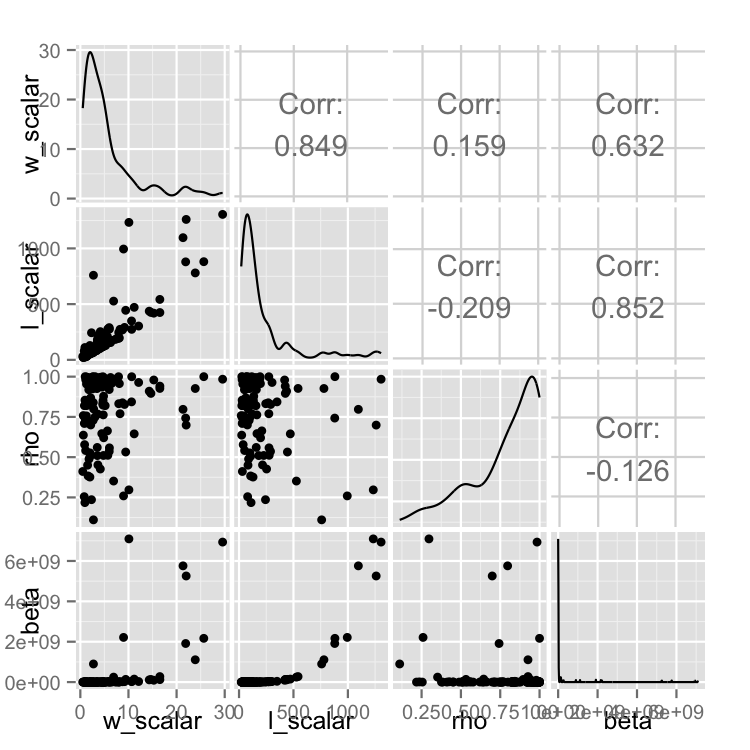
\includegraphics[width=0.7\textwidth]{figure/nondim-fig-1} \hfill{}

\caption[Distribution and correlation of nondimensional parameter estimates]{Distribution and correlation of nondimensional parameter estimates. Shown are the parameter estimates within 20 log-likelihood units of the maximum.}\label{fig:nondim-fig}
\end{figure}


\end{knitrout}

However, another possibility occurs to me, which is that standard DEB theory often works with compound parameters.
In particular, Martin et al., in their 2013 paper that also fit DEB models to growth and reproduction trajectories, defined the DEB model as
\begin{align}
  \frac{dE}{dt} &= \rho \epsilon \mathcal{V} I_{max} \frac{F}{f_h+F} L^g - p_c, \\
  \frac{dL}{dt} &= \frac{1}{3}\left(\frac{v}{gL^2} p_c - k_m L\right), \\
p_c &= L^2 \frac{g e}{g + e}\left(1 + \frac{L k_m}{v}\right).
\end{align}





Another option to address this challenge is to embrace what the data-fitting is saying.
In particular, the data-fitting says that $v$ has no influence on dynamics - I can set it to any value I want without affecting the other parameter estimates, almost at all.
Given that, it makes sense to consider a reserve-less model, which essentially assumes that $v$ is infinite and ingested food is immediately allocated for growth and reproduction.
In this case, the dynamics of the system are simpler:
\begin{align}
\frac{dF}{dt} &= -I_{max} \frac{F}{f_h+F} L^g, \\
\frac{dV}{dt} &= \left(\kappa \rho \epsilon \mathcal{V} I_{max} \frac{F}{f_h+F} L^g - k_m~E_G~V\right)/E_G, \\
\frac{dV}{dt} &= \left((1-\kappa) \rho \epsilon \mathcal{V} I_{max} \frac{F}{f_h+F} L^g\right)/E_R.
\end{align}
I can also do the same nondimensionalization trick to get a slightly simpler system (again moving from volume to length as a state variable):
\begin{align}
\frac{df}{d\tau}&=-\frac{f}{1+f} \ell^g, \\
\frac{d\ell}{d\tau}&=\frac{1}{q}\left(\sigma \phi \frac{f}{1+f}\ell^{g-q+1}-\mu \ell^1\right), \\
\frac{dr}{d\tau}&=\beta\frac{f}{11+f}\ell^g,
\end{align}
where
\begin{align}
\hat{f} &= f_h, \\
\hat{\ell} \text{ is unspecified, and} \\
\hat{\tau} &= \frac{f_h}{I_{max}\hat{\ell}^g}.
\end{align}
Note that the fact that $\hat{\ell}$ is unspecified is a little bit strange, but occurs because there aren't any parameters with units of length; there are only parameters with units of length to some power, such as $I_{max}$ and $\xi$.
The dimensionless parameters are
\begin{align}
\sigma &= \frac{\rho \kappa}{E_G}, \\
\phi &= \frac{f_h \epsilon \mathcal{V}}{\xi \hat{\ell}^q}, \\
\mu &= -k_m \hat{\tau}, \\
\beta &= \frac{\rho (1-\kappa) f_h \epsilon \mathcal{V}}{E_R}.
\end{align}
Here, the things that need to be estimated by the fitting are $\hat{f}$, $\hat{\ell}$, $\sigma$, $\mu$, and $\beta$.
Both $\tau$ and $\phi$ are specified, once $\hat{\ell}$ is specified, as the feeding and length-dry weight regression parameters are all known.

Again, it is not totally clear to me whether this will be an easier estimation problem.



\end{document}
